\section*{Теория}

Рассмотрим условие квазинейтральности с точки зрения средних плотностей заряда. Пусть концентрация ионов равна $n_i$, концентрация электронов -- $n_e$, и каждый ион отдаёт в плазму $Z$ электронов. Тогда условие квазинейтральности запишется в виде:
$$
-en_e + (Ze) n_i = 0, 
$$
$e > 0$ -- элементарный заряд. Далее для простоты изложения будем рассматривать случай однократно ионизованной плазмы $Z = 1$.

\subsection*{Нарушение квазинейтральности плазмы в квазиодномерном случае}

На микроуровне квазинейтральность плазмы может нарушатся из-за тепловых флуктуаций. Отклонение от квазинейтральности может происходить только на малых расстояниях и в течение малых промежутках времени. Оценим характерные расстояния, на которых может происходить разделение зарядов.

\begin{wrapfigure}{left}{0.5\textwidth}
	\vspace{-10pt}
	\centering
	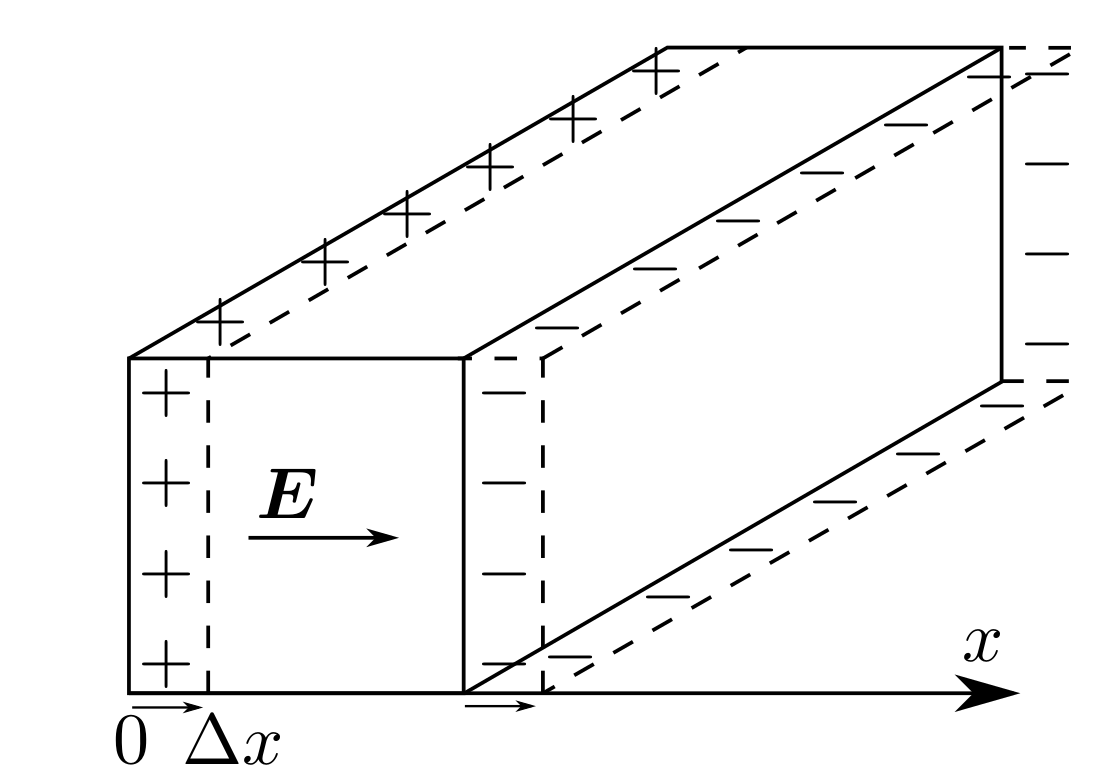
\includegraphics[width=0.48\textwidth]{../res/plasma.png}
	\caption{Плазменные колебания.}
	\label{img:plasma oscil}
\end{wrapfigure}

Пусть в некотором слое толщиной $l$ произошло разделение зарядов. В состоянии равновесия $n_i = n_e \equiv n$. В результате разделения зарядов на боковых плоскостях возникнут нескомпенсированные заряды с плотностью
$$\sigma = \frac{neV}{S} = nel$$
Выделенный слой можно рассматривать как плоский конденсатор. Напряженность электрического поля в плазме будет
$$E = 4\pi \sigma = 4\pi n el$$.
Объёмная плотность энергии такого поля равна
$$\omega_E = \frac{E^2}{8\pi}$$.
Так как электрическое поле было создано разделенными в результате тепловой флуктуации зарядами, то, согласно закону сохранения энергии, кинетическая энергия теплового движения преобразовалась в энергию электрического поля:
$$w_E = w_T$$
По теореме о равнораспределении кинетической энергии по степеням свободы, так как случай одномерный, то
$$
w_T = w_{T}^e + w_{T}^i = n \frac{kT}{2} + n\frac{kT}{2} = nkT
$$
Тогда напряженность поля
$$
E = \sqrt{8nkT}
$$
и толщина слоя
$$
l = \sqrt{\frac{kT}{2\pi n e^2}}
$$
Величину $r_D = \frac{l}{2} = \sqrt{\frac{kT}{8\pi n e^2}}$ называют \textit{дебаевским радиусом} или \textit{дебаевской длиной}. 

Оценим характерное время, в течение которого может происходить разделение зарядов. Рассмотрим смещение $l$ зарядов в слое плазмы (рис. \ref{img:plasma oscil}). На электроны действует электрическое поле:
$$
E = 4 \pi n e l
$$
Запишем уравнение движения электронов:
$$m \ddot{l} = -4 \pi n e^2 l$$
Это уравнение, решением которого является гармонический осциллятор с частотой $\omega_p = \sqrt{\frac{4\pi n e^2}{m}}$, называемой \textit{ленгмюровской} или \textit{плазменной}. 

Таким образом, ленгмюровская частота $\omega_p$ определяет время отклика плазмы на флуктуацию заряда, а дебаевский радиус определяет характерные размеры флуктуаций. То есть ленгмюровская частота и дебаевский радиус характеризуют временной и пространственный масштаб плазменных явлений.

Теперь можно дать количественное описание коллективного характера взаимодействия плазмы. Плазмой можно считать газ, дебаевский радиус которого много меньше характерного размера области $d$, занимаемой газом:
$$
r_D = \sqrt{\frac{kT}{8 \pi n e^2}} \ll d
$$
Если характерный размер области меньше дебаевского радиуса, то тепловые флуктуации будут оказывать более значительное влияние, чем электромагнитные взаимодействия. Тогда можно будет рассматривать только взаимодействия частиц во время столкновений, а дальнодействующими силами пренебречь.

\subsection*{Плазменное экранирование}

Внесем в плазму точеный заряд $q$. Под действием внешнего поля электроны в плазме перераспределяться так, чтобы скомпенсировать поле точеного заряда. Из-за наличия тепловых флуктуаций полной нейтрализации поля заряда наблюдаться не будет. Ослабление внешнего поля в плазме называется \textit{экранированием}.

Потенциал точечного заряда равен
$$\phi_q = \frac{q}{r}$$
В плазме потенциал 

\subsection*{Идеальная и не идеальная плазмы}

Рассмотрим \textit{дебаевскую сферу} -- область в плазме, ограниченную сферой радиуса $$r_D$$. Концентрация частиц в сфере
$$N = \frac{4}{3} \pi r_D^3 n$$
В веществе объемом $V$ и концентрацией частиц $n$ находится $N = nV$ частиц, тогда каждая частица в среднем занимает объем $V_0 = \frac{V}{N} = \frac{1}{n} \sim d^3$, поэтому среднее расстояние между частицами $d \sim n^{-1/3}$. Тогда 
$$N \sim \left( \frac{r_d}{d} \right)^3$$

Рассмотрим два предельных случая.
\begin{enumerate}
	\item $N \gg 1$. То есть в дебаевской сфере находится очень много частиц. Так как экранирование на расстояниях порядка дебаевского радиуса $r_D$ невелико, то заряженные частицы будут проявлять коллективные эффекты, связанные с электромагнитным взаимодействием. Заметим, что хотя количество частиц в сфере велико, плазма является \textit{разреженной} из-за большого дебаевского радиуса:
	$$
	r_D \sim \sqrt{\frac{kT}{8 \pi n e^2}} \gg n^{-1/3} \Rightarrow n \ll \left( \frac{kT}{e^2} \right)^3
	$$
	Покажем, что потенциальная энергия взаимодействия частиц мала по сравнению с их кинетической энергией. Условие разреженной плазмы можно переписать в виде:
	$$w_E \sim \frac{e^2}{d} \ll w_T \sim kT$$
	Плазму называют \textit{идеальной}, если потенциальная энергия взаимодействия частиц мала по сравнению с кинетической энергией. В данном случае плазму с хорошей точностью можно рассматривать как идеальный газ.
	
	\item $N \ll 1$. Из-за малого дебаевского радиуса, плотность плазмы велика:
	$$n \gg \left( \frac{kT}{e^2} \right)^3$$
	Такую плазму называют \textit{плотной}, и её нельзя рассматривать как идеальный газ.
\end{enumerate}

